\chapter{Contexte}

\section{Le secrétariat social Sodabel}

\begin{figure}[H]
    \centering
    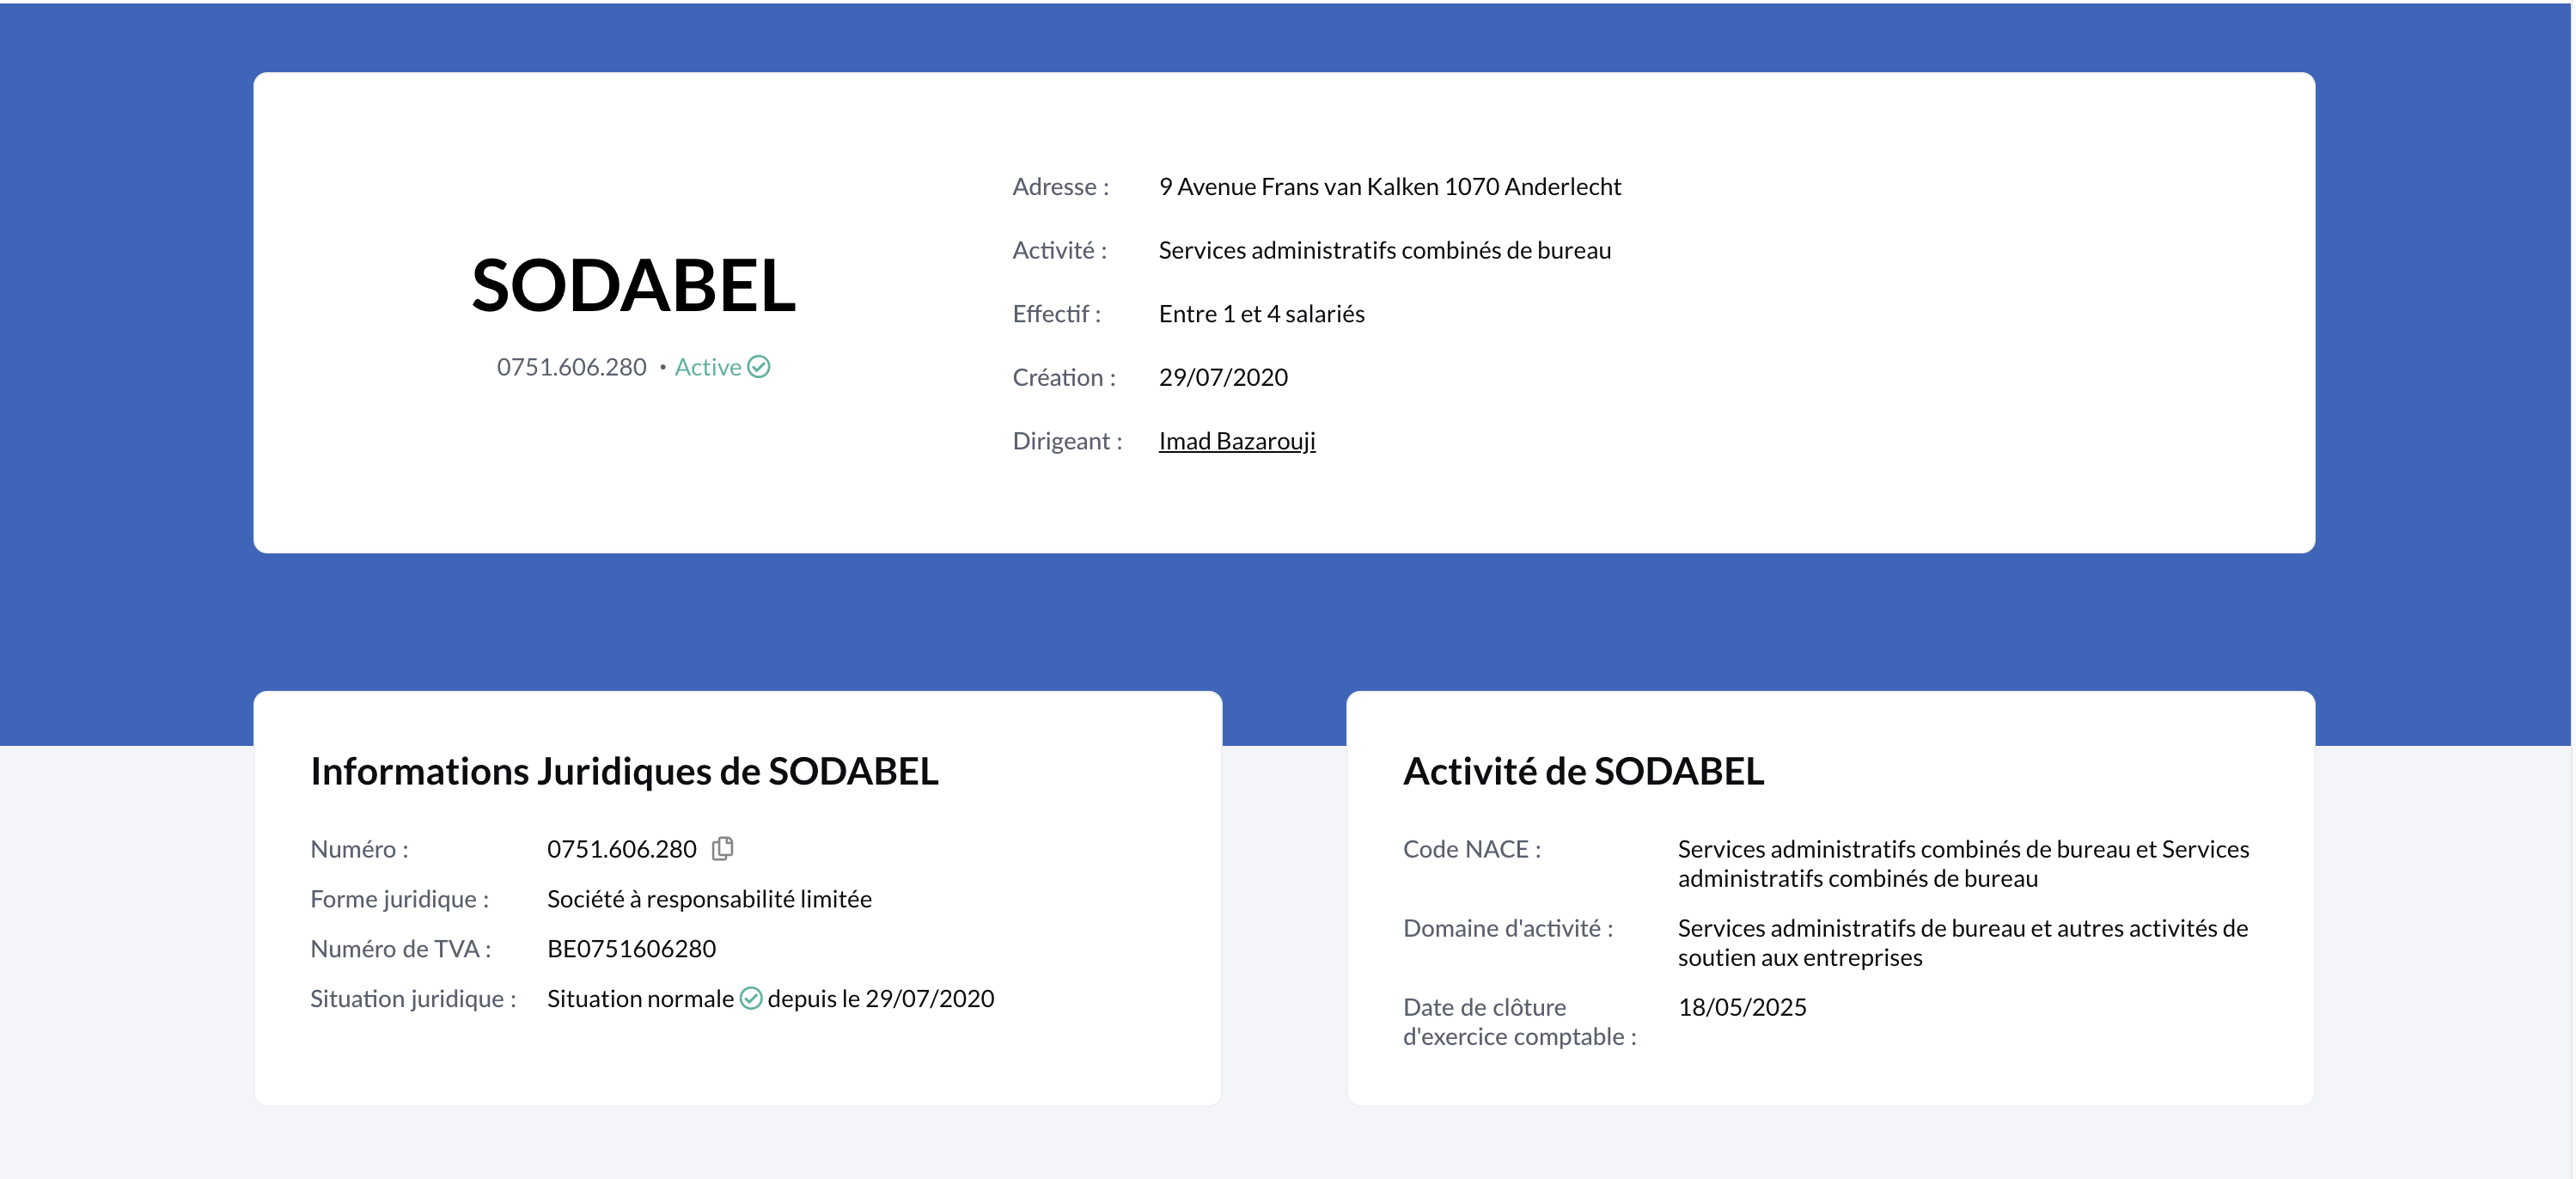
\includegraphics[width=0.9\textwidth]{sodabelInfos.png}
    \caption{Informations sur le secrétariat social Sodabel \cite{pappers-sodabel}}
    \label{fig:sodabelInfos}
\end{figure}

\begin{tcolorbox}[
  title={\textbf{Profil de Sodabel}},
  colback=blue!5!white,
  colframe=primarycolor,
  fonttitle=\bfseries,
  boxrule=0.5mm,
  arc=2mm,
  left=6mm,
  right=6mm,
  top=6mm,
  bottom=6mm
]
\noindent\textbf{Sodabel} est un secrétariat social indépendant qui offre une gamme complète de services administratifs aux petites entreprises et indépendants, en collaboration avec \textbf{FiscoFid} pour les services comptables complémentaires. 

\noindent Ces deux entreprises sont gérées par le même dirigeant, créant ainsi un écosystème de support administratif complet pour leurs clients.

Sa clientèle est principalement composée d'indépendants et de petites entreprises issues de secteurs variés, avec une forte représentation dans les domaines du :
\begin{itemize}[leftmargin=*,label=\textcolor{darkgray}{$\bullet$},itemsep=0.3em]
  \item \textbf{Transport} (taxis)
  \item \textbf{Restauration}
  \item \textbf{Construction}
\end{itemize}
\end{tcolorbox}

\section{Problématique et besoins}

Malgré son expertise dans le domaine du secrétariat social, Sodabel fait face à plusieurs défis opérationnels liés à ses processus actuels, majoritairement manuels. L'absence d'un système informatique dédié engendre des inefficacités et des risques qui impactent tant la qualité du service que la satisfaction client.

\noindent Les principaux problèmes identifiés sont :

\begin{itemize}[leftmargin=*,label=\textcolor{darkgray}{$\bullet$},itemsep=0.3em]
  \item \textbf{Saisie manuelle des données} lors de la déclaration des collaborateurs, particulièrement sujette aux erreurs. Une simple faute de frappe ou une mauvaise interprétation des informations transmises peut avoir des conséquences significatives, entraînant des complications légales et administratives.
  
  \item \textbf{Communication fragmentée} entre Sodabel et ses clients. L'utilisation de canaux multiples et non structurés (visites en personne, emails, messages WhatsApp) pour la transmission d'informations critiques crée un environnement propice aux malentendus et aux oublis.
  
  \item \textbf{Absence de système de suivi} des déclarations DIMONA. Actuellement, Sodabel ne dispose d'aucun système centralisé permettant de suivre et de mettre à jour manuellement le statut des déclarations soumises à l'Office National de Sécurité Sociale (ONSS).
\end{itemize}

\noindent Ces différentes problématiques soulignent un besoin clair de digitalisation des processus au sein de Sodabel, afin de réduire les risques d'erreurs, d'améliorer l'efficacité opérationnelle et d'offrir un meilleur service à ses clients.

\section{Processus métier}

Pour mieux comprendre les enjeux et les opportunités d'amélioration, il est essentiel d'examiner en détail les principaux processus métier actuellement en place chez Sodabel.

\subsection{Processus de création d'une entreprise cliente}

Lorsqu'une nouvelle entreprise souhaite devenir cliente de Sodabel, le processus actuel est entièrement manuel. L'entreprise doit se présenter physiquement au secrétariat social ou envoyer les informations requises par email ou WhatsApp. Une secrétaire de Sodabel collecte alors manuellement toutes les données nécessaires : informations d'identification de l'entreprise, coordonnées du responsable, secteur d'activité, nombre d'employés prévus, etc.

\noindent Ce processus présente plusieurs inconvénients :
\begin{itemize}[leftmargin=*,label=\textcolor{darkgray}{$\bullet$},itemsep=0.3em]
  \item Risque élevé d'erreurs lors de la transcription des données
  \item Temps de traitement important
  \item Difficulté à retrouver et à mettre à jour les informations
  \item Absence de validation automatique des données saisies
\end{itemize}

\subsection{Processus d'ajout d'un collaborateur}

L'ajout d'un nouveau collaborateur pour une entreprise cliente suit un schéma similaire. L'entreprise communique les informations du collaborateur soit en personne, soit par voie électronique (email, WhatsApp). Une secrétaire de Sodabel doit alors saisir manuellement ces données pour préparer les documents nécessaires et effectuer les déclarations obligatoires.

\begin{note}
Ce processus est particulièrement critique car les erreurs à ce niveau peuvent avoir des conséquences légales importantes. Une erreur dans la saisie du numéro de registre national, de la date de début de contrat ou du type de contrat peut entraîner des problèmes administratifs significatifs tant pour l'employeur que pour l'employé.
\end{note}

\subsection{Processus de déclaration DIMONA}

La Déclaration Immédiate/Onmiddellijke Aangifte (\textbf{DIMONA}) est une obligation légale en Belgique qui consiste à déclarer immédiatement tout engagement ou fin de relation de travail auprès de l'ONSS. Chez Sodabel, ce processus est actuellement géré de manière réactive.

\noindent Lorsqu'une entreprise cliente souhaite déclarer un nouveau collaborateur, elle fournit les informations nécessaires à Sodabel. Une secrétaire saisit alors ces informations dans le système de l'ONSS pour effectuer la déclaration DIMONA. Cependant, il n'existe aucun système interne permettant de suivre et de mettre à jour manuellement le statut de ces déclarations.

\noindent Cette approche présente plusieurs inconvénients :
\begin{itemize}[leftmargin=*,label=\textcolor{darkgray}{$\bullet$},itemsep=0.3em]
  \item Absence d'un système centralisé pour suivre le statut des déclarations
  \item Impossibilité de mettre à jour manuellement le statut des déclarations dans un système dédié
  \item Difficulté à fournir des informations actualisées aux clients
  \item Risque accru de non-conformité avec les obligations légales
\end{itemize}

\vspace{1cm}

\begin{tcolorbox}[
  title={\textbf{Solution proposée : SecuCom}},
  colback=blue!5!white,
  colframe=primarycolor,
  fonttitle=\bfseries,
  boxrule=0.5mm,
  arc=2mm,
  left=6mm,
  right=6mm,
  top=6mm,
  bottom=6mm
]
\noindent L'ensemble de ces processus métier, bien que fonctionnels, présente des inefficacités et des risques qui justifient pleinement le développement d'une solution informatique dédiée comme \textbf{SecuCom}.\\

\noindent Cette plateforme vise à :
\begin{itemize}[leftmargin=*,label=\textcolor{darkgray}{$\bullet$},itemsep=0.3em]
  \item \textbf{Digitaliser} les processus administratifs
  \item \textbf{Permettre un suivi manuel} des déclarations DIMONA
  \item \textbf{Réduire} les risques d'erreurs
  \item \textbf{Améliorer} l'efficacité opérationnelle
  \item \textbf{Augmenter} la qualité du service offert par Sodabel à ses clients
\end{itemize}
\end{tcolorbox}
